\subsection{Analytics Module}
\label{sec:mobile-analytics}

\textbf{Purpose:}
Provides users with analytical insights into workflow performance and execution history. The Analytics module enables users to monitor workflow activities, evaluate execution trends, and review previous operations through an intuitive visual interface.

\vspace{0.2cm}
\noindent\textbf{Main Features}

\begin{itemize}
    \item Workflow Statistics
    \item Performance Insights
    \item Execution History
    \item Activity Monitoring
\end{itemize}

%%%%%%%%%%%%%%%%%%%%%%%%%%%%%%%%%%%%%%%%%%%%%%%%%%%%%%%%%%%%

\subsubsection{Insights Dashboard}

\textbf{Purpose:}
Presents summarized statistics and performance metrics that help users monitor the overall status of workflow automation projects.

\begin{figure}[H]
    \centering
    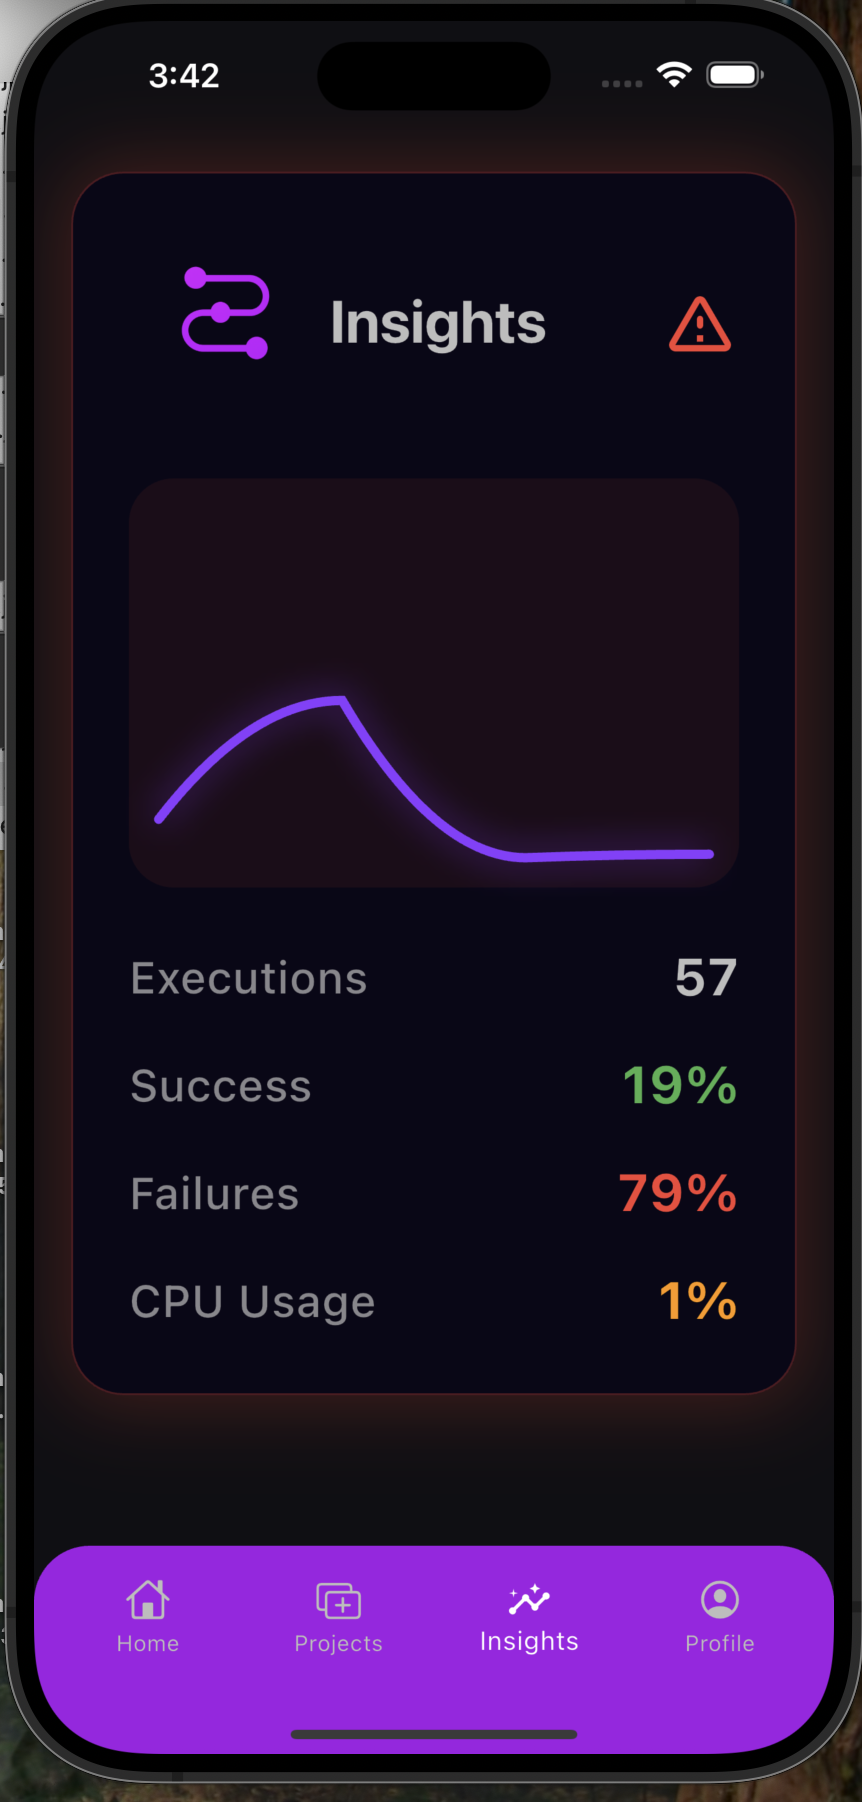
\includegraphics[width=0.42\textwidth]{images/mobile-app/admin-dashboard/insights-page-D.png}
    \caption{Insights Dashboard}
    \label{fig:mobile-insights}
\end{figure}

\vspace{0.2cm}
\noindent\textbf{Main Components}

\begin{itemize}
    \item Statistics Cards
    \item Workflow Performance Summary
    \item Activity Overview
    \item Refresh Action
\end{itemize}

\vspace{0.2cm}
\noindent\textbf{Behavior \& Logical Flows}

\begin{itemize}
    \item Retrieves analytics information from the backend through authenticated REST API requests.
    \item Displays workflow statistics in an organized dashboard.
    \item Updates the displayed analytics after workflow execution changes.
    \item Highlights active and inactive workflows for quick monitoring.
    \item Displays loading indicators while analytics data is being fetched.
\end{itemize}

%%%%%%%%%%%%%%%%%%%%%%%%%%%%%%%%%%%%%%%%%%%%%%%%%%%%%%%%%%%%

\subsubsection{History Screen}

\textbf{Purpose:}
Displays a chronological record of workflow executions, allowing users to review previous operations and monitor recent system activities.

\begin{figure}[H]
    \centering
    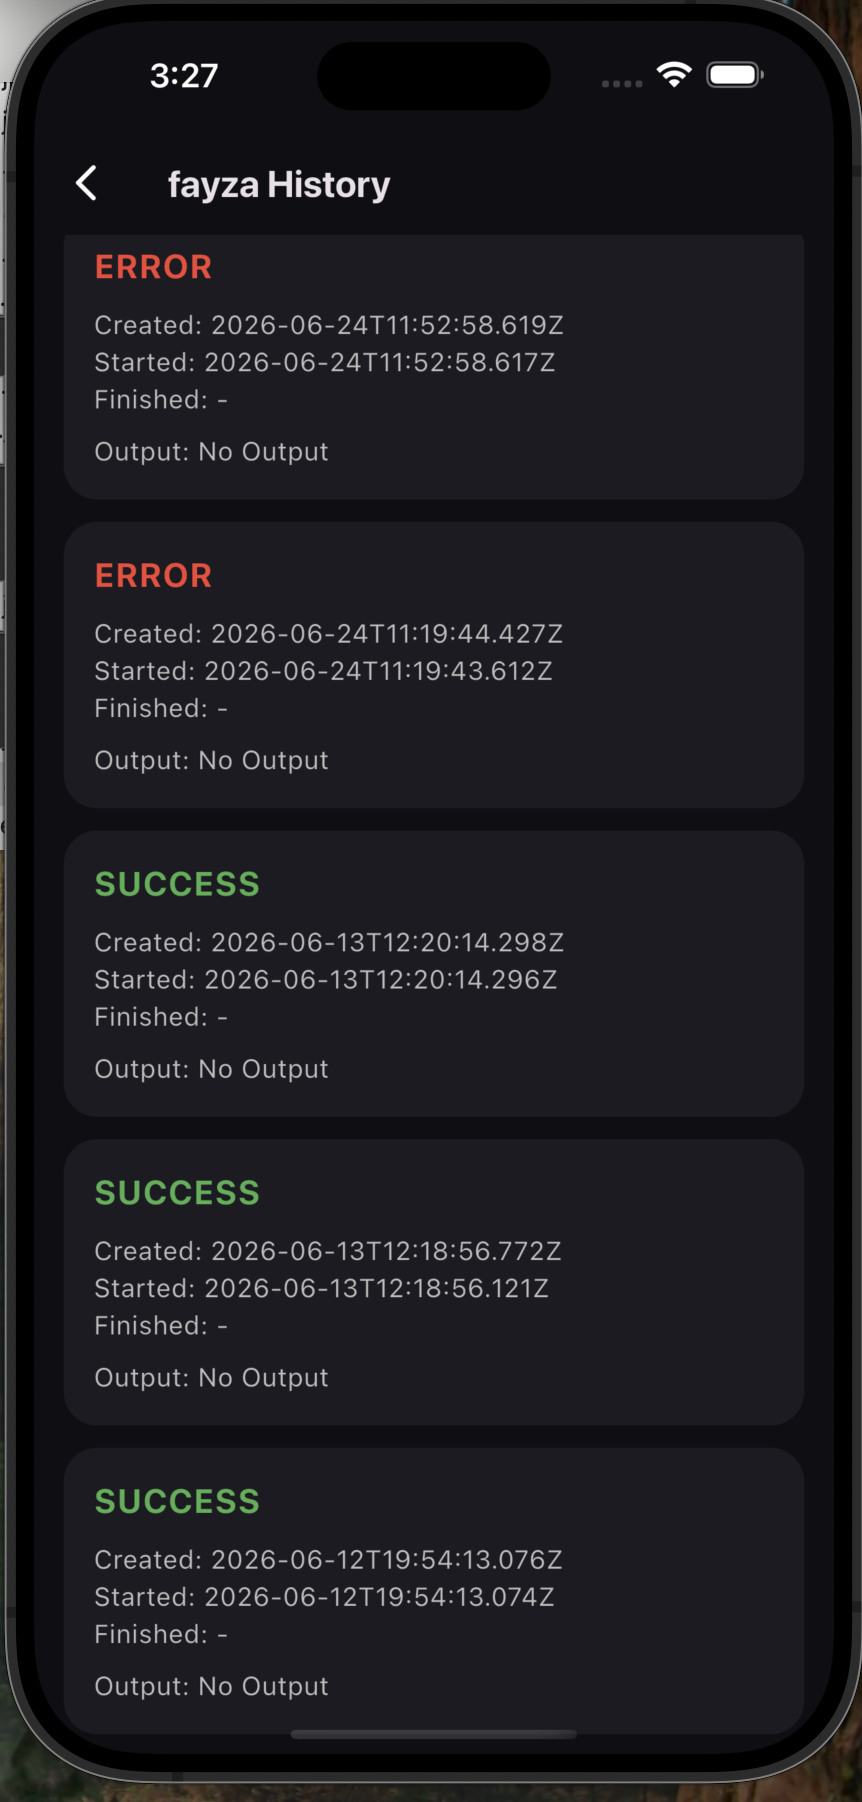
\includegraphics[width=0.42\textwidth]{images/mobile-app/admin-dashboard/history-page-D.png}
    \caption{Workflow History}
    \label{fig:mobile-history}
\end{figure}

\vspace{0.2cm}
\noindent\textbf{Main Components}

\begin{itemize}
    \item Activity List
    \item Execution Status
    \item Execution Timestamp
    \item Pull-to-Refresh
\end{itemize}

\vspace{0.2cm}
\noindent\textbf{Behavior \& Logical Flows}

\begin{itemize}
    \item Retrieves workflow execution history from the backend.
    \item Displays executions in reverse chronological order.
    \item Shows the execution status for each workflow.
    \item Refreshes the history after successful workflow operations.
    \item Handles loading and error states to improve the user experience.
\end{itemize}

%%%%%%%%%%%%%%%%%%%%%%%%%%%%%%%%%%%%%%%%%%%%%%%%%%%%%%%%%%%%

\subsubsection{Data Synchronization}

\textbf{Purpose:}
Maintains synchronization between the mobile application and backend services to ensure analytics and history data remain up to date.

\vspace{0.2cm}
\noindent\textbf{Behavior \& Logical Flows}

\begin{itemize}
    \item Sends authenticated API requests using the stored JWT access token.
    \item Refreshes analytics automatically after workflow deployment or termination.
    \item Synchronizes workflow history whenever new executions are completed.
    \item Displays loading indicators while data is being retrieved.
    \item Ensures consistency between backend data and the mobile user interface.
\end{itemize}